\section{Desarrollo}
%Deben explicarse los métodos numéricos que utilizaron y su aplicación al problema
%concreto involucrado en el trabajo práctico. Se deben mencionar los pasos que si-
%guieron para implementar los algoritmos, las dificultades que fueron encontrando y la
%descripción de cómo las fueron resolviendo. Explicar también cómo fueron planteadas
%y realizadas las mediciones experimentales. Los ensayos fallidos, hipótesis y conjeturas
%equivocadas, experimentos y métodos malogrados deben figurar en esta sección, con
%una breve explicación de los motivos de estas fallas (en caso de ser conocidas).

\subsection{Planteo del Problema}
Como dijimos anteriormente en nuestro problema teníamos un parabrisas con infinitos puntos, por ser una superficie continua, una forma de pensar el problema es discretizar estos puntos, y trabajar sobre ello. Una vez hecha esta operación, podemos modelar los puntos resultantes con una matriz, donde cada posición de esta matriz represente un punto en el parabrisas. Para simplificar como los bordes del parabrisas tienen una temperatura constante de -100. Estos puntos no se representan en el parabrisas discretizado. Por lo que tampoco en la matriz asociada. \newline
Al discretizar los puntos, para obtener las temperaturas en cada punto restante del parabrisas continuo utilizaremos la formula:
$$
t_{ij} = \frac{t_{i-1,j} + t_{i+1,j} + t_{i,j-1} + t_{i,j+1}}{4}
$$

En nuestro problema nos interesa conocer el punto crítico (el centro del parabrisas), esto además significa conocer la temperatura de sus vecinos, y a su vez los vecinos necesitaran conocer la temperatura de sus otros vecinos.
Es decir que en un principio es necesario calcular la temperatura de todos los puntos del parabrisas discretizado.
Este problema es modelado mediante un sistema de ecuaciones, en el cual cada ecuación se corresponde con un solo punto del parabrisas. Dicho sistema de ecuaciones lo representamos en una matriz cuyo tamaño es $\#puntos$ x $\#puntos$. Finalmente podemos calcular la temperatura en cada punto aplicando \textit{eliminación gaussiana} sobre la matriz.

Una vez que sabemos qué temperatura hay en el punto crítico, podremos decidir que criterio utilizar para matar sanguijuelas, mediante distintas experimentaciones.


\subsection{Nuestro sistema de ecuaciones.}

Con el objetivo de calcular la temperatura de cada punto de nuestra matriz de $n\times m$, la cual es una representación discreta del parabrisas de largo $b$, ancho $a$ y granularidad $h$. En nuestro problema inicial, planteamos un sistema de ecuaciones compuesto por $n*m$ incógnitas (una por cada punto con 1 $<=$ n $<=$ ($a/h$ -1), 1 $<=$ m $<=$ ($b/h -1$)). Con este motivo, numeramos los puntos $(i,j)$ del parabrisas mediante la función:\\

\begin{equation}
	F(i, j) = i*m + j, \quad F(i,j) \in [1, n*m]
\end{equation}\\

Además, como se mencionó anteriormente, para cada punto $\alpha_{i,j}$ en el parabrisas se le corresponde una de las siguientes ecuaciones:


  \begin{itemize}
    \item 	$T_{\alpha}$ = -100 $\quad \quad$ si: i = 0 $\vee$ i = $a/h$ $\vee$ j = b $\vee$ j = $b/h$\newline
    \item 	$T_{\alpha}$ = $T_{Sanguijuela}$ $\quad \quad$ si: $(i,j)$ $\in$ Sanguijuela \newline
  	  \item 	$4T_{\alpha}$ - $T_{\alpha+1}$ -$T_{\alpha-1}$- $T_{\alpha+m}$- $T_{\alpha-m}$ = 0 \quad \quad Demás casos\newline
  \end{itemize}

Finalmente, representamos el sistema de las ecuaciones $(1,\ldots, n*m)$ como la matriz extendida de $Ax=B$.
A modo de ejemplo la representación del sistema de ecuaciones de un parabrisas discretizado de $4\times 4$:

\setcounter{MaxMatrixCols}{20}


\[ \left( \begin{matrix}
4 & -1 & 0 & 0 & -1 & 0 & 0 & 0 & 0 & 0 & 0 & 0 & 0 & 0 & 0 & 0 & | &-200\\
-1 & 4 & -1 & 0 & 0 & -1 & 0 & 0 & 0 & 0 & 0 & 0 & 0 & 0 & 0 & 0 & | &-100\\
0 & -1 & 4 & -1 & 0 & 0 & -1 & 0 & 0 & 0 & 0 & 0 & 0 & 0 & 0 & 0 & | &-200\\
0 & 0 & -1 & 4 & 0 & 0 & 0 & -1 & 0 & 0 & 0 & 0 & 0 & 0 & 0 & 0 & | &-100\\
-1 & 0 & 0 & 0 & 4 & -1 & 0 & 0 & -1 & 0 & 0 & 0 & 0 & 0 & 0 & 0 & | &-100\\
0 & -1 & 0 & 0 & -1 & 4 & -1 & 0 & 0 & -1 & 0 & 0 & 0 & 0 & 0 & 0 & | & 0\\
0 & 0 & 0 & 0 & 0 & 0 & 1 & 0 & 0 & 0 & 0 & 0 & 0 & 0 & 0 & 0 & | & T_{Sang1}\\
0 & 0 & 0 & 0 & 0 & 0 & -1 & 4 & 0 & 0 & 0 & -1 & 0 & 0 & 0 & 0 & | &-100\\
0 & 0 & 0 & 0 & 0 & 0 & 0 & 0 & 4 & -1 & 0 & 0 & -1 & 0 & 0 & 0 & | &-100\\
0 & 0 & 0 & 0 & 0 & 0 & 0 & 0 & 0 & 1 & 0 & 0 & 0 & 0 & 0 & 0 & | &T_{Sang2}\\
0 & 0 & 0 & 0 & 0 & 0 & -1 & 0 & 0 & -1 & 4 & -1 & 0 & 0 & -1 & 0 & | &0\\
0 & 0 & 0 & 0 & 0 & 0 & 0 & 0 & 0 & 0 & -1 & 4 & 0 & 0 & 0 & -1 & | &-100\\
0 & 0 & 0 & 0 & 0 & 0 & 0 & 0 & -1 & 0 & 0 & 0 & 4 & -1 & 0 & 0 & | &-200\\
0 & 0 & 0 & 0 & 0 & 0 & 0 & 0 & 0 & -1 & 0 & 0 & -1 & 4 & -1 & 0 & | &-100\\
0 & 0 & 0 & 0 & 0 & 0 & 0 & 0 & 0 & 0 & -1 & 0 & 0 & -1 & 4 & -1 & | &-100\\
0 & 0 & 0 & 0 & 0 & 0 & 0 & 0 & 0 & 0 & 0 & -1 & 0 & 0 & -1 & 4 & | &-200\\

\end{matrix} \right)\] 
\textit{En este ejemplo se representa un parabrisas discretizado con dos sanguijuelas}


\subsection{¿Por qué una matriz Banda?}
La obtención de la matriz Banda esta ligada directamente con nuestro sistema de ecuaciones, con la ecuación de calor discretizada y con el orden de numeración de las variables. \\
Por ejemplo, la siguiente figura  muestra un ejemplo de instancia de un parabrisa:

    \begin{figure}[H]
    \centering
    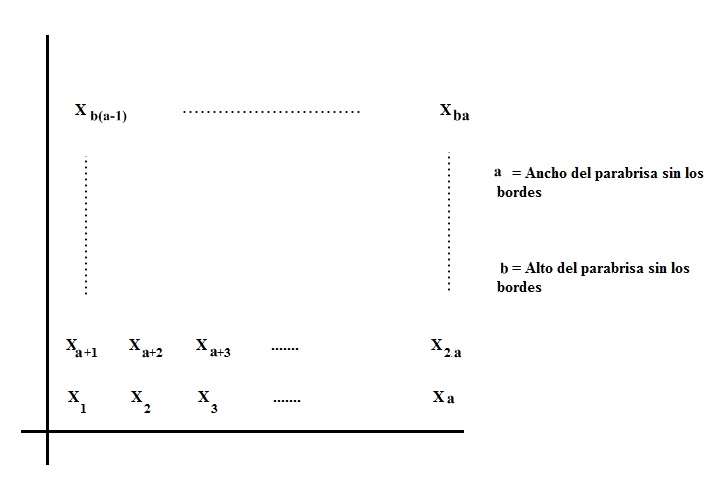
\includegraphics[scale=0.7]{graphs/mapa.jpg}\caption{Cada X$_i$ representa un punto de la discretizacin de este parabrisa}
      \end{figure}
      
      
      
Empezemos a despejar las variables y armar nuestro sistema de ecuaciones:\\
    \begin{itemize}
    \item  X$_1$ = (X$_2$ + X$_{a+1}$ - 100 - 100)/4\\
            4*X$_1$ - X$_2$ - X$_{a+1}$ = -200 
            
    \item X$_2$ = (X$_1$ + X$_{a+2}$ + X$_3$ - 100)/4\\
            4*X$_2$ - X$_1$ - X$_{a+2}$ - X$_3$ = -100 
    
    \end{itemize}
    
    Así, sucesivamente hasta despejar todas las incógnitas y completar el sistema. Como consecuencia del uso de la ecuación de calor, cada incógnita va a depender de una incógnita que este a la izquierda, derecha, arriba, y abajo de la misma. Esto se interpreta como que cada una de las variables, se relaciona con a lo sumo dos variable pegadas y con dos variable que están a A de distancia de la variable en estudio (Decimos a lo sumo, para especificar el caso de las variables que estás pegadas a los bordes, o sanguijuelas). Esto, y que empezamos despejando desde el extremo inferior izquierdo del parabrisa, son las causas de que la matriz quede establecida como una matriz banda.\\
    Armando la matriz asociada al sistema de ecuaciones, nos da como resultado la siguiente figura, que muestra la relación de las variables con la distancia A.
    
        \begin{figure}[H]
    \centering
    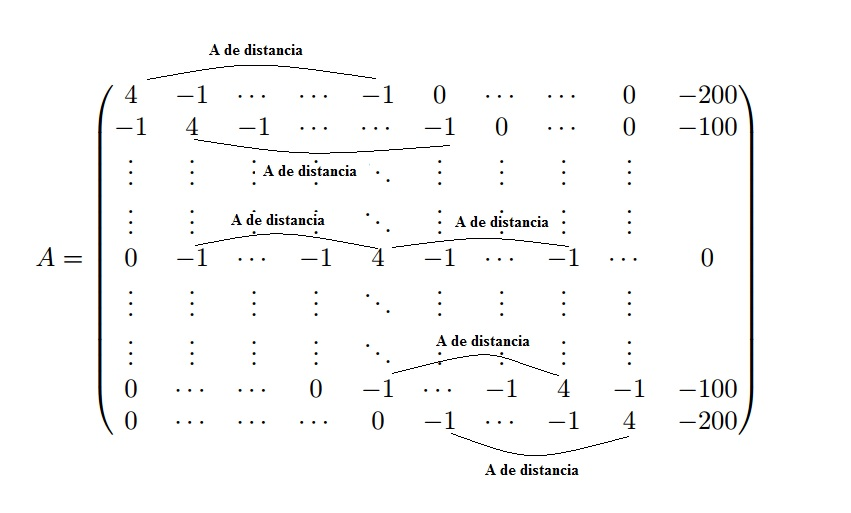
\includegraphics[scale=0.7]{graphs/matriz.jpg}
      \end{figure}
    
    

\subsection{Estructura de la matriz bandas}
Para representar el sistema de ecuaciones, vamos a implementar una estructura que trabaja internamente con una matriz, la cual guarda únicamente los elementos del sistema que nos interesan. Recordemos primero, que dados $a, b$ y $h$, $n = a/h$, $m = b/h$ entonces estaremos discretizando $(n + 1)$x$(m + 1)$ puntos. 
Dado que hay $(n + 1)$x$(m + 1)$ puntos a los cuales debemos asociarles sus respectivas temperaturas, como sabemos a priori que los bordes tienen una temperatura constante de -100, en realidad nos van a interesar las temperaturas de los demás puntos, es decir de $(n - 1)$x$(m - 1)$ puntos (ya que hay dos bordes horizontales y dos verticales). Sabemos entonces, que si tenemos $(n - 1)$x$(m - 1)$ puntos a los cuales debemos asociarles temperaturas, vamos a tener $(n - 1)$x$(m - 1)$ incógnitas y también $(n - 1)$x$(m - 1)$ ecuaciones lineales. La idea es aprovechar que la matriz asociada al sistema de ecuaciones tiene la forma de una matriz bandas, usando esto a nuestro favor para reducir la complejidad espacial que requiere el problema.
\par La idea es utilizar como dijimos antes, una matriz que represente el sistema de ecuaciones. Para hacer esto, no vamos a poder evitar tener $(n - 1)$x$(m - 1)$ filas debido a que cada fila va a representar cada punto de la discretización. Lo que sí se puede evitar, es tener $(n - 1)$x$(m - 1)$ columnas ya que, al tratarse de una matriz bandas, la ecuación $i$ que representa al punto $X_i$ va a usar a lo sumo a los puntos $X_{i - (m - 1)}$, $X_{i + (m - 1)}$, $X_{i + 1}$ y $X_{i - 1}$. Entonces como sucede esto, con tener $2$x$(m - 1) + 2$ columnas es suficiente. Las dos columnas adicionales que contamos se deben a que necesitamos en cada fila poder representar el valor valor correspondiente al coeficiente del punto $X_i$ y, dado que vamos a guardar la matriz asociada al sistema, ésta va a ser de la forma $A|b$, por lo tanto necesitamos una columna más para los elementos de $b$. Utilizando una matriz de estas dimensiones, nuestra complejidad espacial para representar el sistema pasa de ser $O((n - 1)^2(m - 1)^2)$ a ser $O((n - 1)(m - 1)^2)$.
\par Hasta ahora lo que explicamos es simplemente que es posible almacenar la matriz asociada al sistema de ecuaciones de una manera más eficiente que guardándola todos sus valores. En nuestra implementación, lo que hicimos es que la estructura que representa el sistema de ecuaciones, mantenga privada esta matriz de $(n - 1)$x$(2(m - 1) + 2)$ de manera tal que cuando queramos acceder a un elemento de la matriz que representa lo hagamos como si estuvieramos tratando con la matriz entera. Para esto, es necesario poder "mapear" de alguna manera cada elemento de la matriz asociada al sistema de ecuaciones, a la matriz que utiliza internamente nuestra estructura para representarla. Explicaremos a continuación, la lógica detrás del mapeo este:
\newline Sea $A_{ij}$ $1 \leq i \leq n - 1, 1 \leq j \leq m - 1$ un elemento de la matriz asociada al sistema de ecuaciones que queremos resolver $A \in \mathbb{R}^{(n - 1)x(m - 1)}$ y sea $A' \in \mathbb{R}^{(n - 1)x(2(m - 1) + 2)}$ la matriz interna que utiliza nuestra estructura para representar a $A$:
\begin{itemize}
\item Si $i = j$, entonces $A_{ij} = A'_{i (m + 1)}$ debido a que estamos tratando de acceder al coeficiente de la incógnita correspondiente a la fila $i$ y, por una cuestión de implementación decidimos situarlo en el medio de cada fila.
\item Si $j = m - 1$ entonces $A_{ij} = A'_{ij}$ ya que estamos tratando de acceder a un $b_i$ y el vector $b$ de resultados de las ecuaciones queda almacenado de manera intacta.
\item Si $j > i$ estamos tratando de acceder a un elemento que está a la derecha (en nuestra matriz interna) del elemento que almacena el coeficiente de la incógnita correspondiente a esta fila
\begin{itemize}
\item Si $j - i \leq m - 1$ entonces quiere decir que tenemos almacenado a este elemento y por lo tanto $A_{ij} = A'_{i, m + j - i}$
\item Caso contrario $A_{ij} = 0$ ya que estamos tratando de acceder al coeficiente (en la ecuación $i$) de un punto que seguro esta ecuación no utiliza.
\end{itemize}
\item Si $j < i$ estamos tratando de acceder a un elemento que está a la izquierda (en nuestra matriz interna) del elemento que almacena el coeficiente de la incógnita correspondiente a esta fila.
\begin{itemize}
\item Si $j - i \leq m - 1$ entonces quiere decir que tenemos almacenado a este elemento y por lo tanto $A_{ij} = A'_{i, m - (i - j)}$.
\item Caso contrario $A_{ij} = 0$ ya que estamos tratando de acceder al coeficiente de un punto que seguro esta ecuación no utiliza.
\end{itemize}
\end{itemize}




\subsection{Eliminacion Gaussiana para matriz Banda}
Algorítmicamente, la idea es similar a la Eliminacion Gaussiana clásica. En este caso, como consecuencia de nuestro sistema de ecuaciones, la matriz resultante del sistema asociado se compone por una diagonal integrada:
\begin{itemize}
\item Por números 4, si se trata de una posicion sin sanguijuela.
\item Por números 1, si se trata de una posición con sanguijuela.
\end{itemize}

Las demás posiciones de la matriz se llenan con -1 o 0, depende el caso.\\ 
Aprovechando las características de la diagonal y los posibles números, no es necesario intercambiar filas debido a que, al triangular, la diagonal nunca va a tener números 0. Además, ya que estas matrices tienen la cualidad de tener diagonales de 0 en los extremos superior derecho e inferior izquierdo nos simplifica las siguiente operacion en relación al algoritmo clásico:

\begin{itemize}
\item No es necesario restar la fila completa, por la presencia de números 0 en el extremo superior derecho.
\item Por cada paso que avanzo en la diagonal, no es necesario realizar la resta de filas hasta abajo, por la presencia de 0 en el extremo inferior izquierdo  
\end{itemize}

Además, en el momento de ir consiguiendo los número 0 de la triangulación, se los asigna directamente para no tener problemas de precisión. Resumiendo, el codigo quedaría asi:\\

\begin{algorithm}[H]
\caption{EliminacionGaussiana0()}
\begin{algorithmic}[1]

\For{$j = 0; filas; j++$}
    \For{$(i = j+1; (i <= j + ancho) \&\&  (i < filas); i++)$}
        \State coeficiente  = (Obtener(i,j)/Obtener(j,j));
		\State  RestarFila0(coeficiente, j, i, j+1);
	\EndFor 
    		\State cerosAIzquierda(j,j);
\EndFor

\end{algorithmic}
\end{algorithm}





\textit{Siendo ancho, el ancho del parabrisa, es decir el ancho de la banda, filas la cantidad de filas de la matriz y restarFila0 es la función para restar filas con la particularidad de lo expresado anteriormente}
	
\subsection{BackWard Substitution para matriz Banda}
Aprovechando la estructura de las matrices bandas, al aplicar Eliminación Gaussiana, la matriz triangular superior resultante hereda las bandas superiores de 0. Ante esto el algoritmo clásico de BackWard Substitution se puede modificar para aprovechando que algunos valores con 0. El caso de ForWard Substitution es análogo



\subsection{Matriz LU para matriz Banda}

Consideremos A una matriz banda, A $\in$ $\Re^{nxn}$, con $b_s$ y $b_i$ las bandas superiores e inferiores correspondientemente y $b_s$ $=$ d, $b_i$ $=$ d.\newline
Al momento de representar la matriz LU de A, se aprovechó que la misma fuese bandas. Ya que entonces, la matriz LU hereda el número de bandas de A. Para la matriz L, esto se puede ver al momento de aplicar la Eliminación Gaussiana en una matriz de este tipo. Si desarrollamos el primer paso de la eliminacion Gaussaiana lo que se  realiza es la diferencia entre $F_i$ - $(a_{1,1}/a_{i,1})1*F_1$, $\forall$ $2 <= i <= d+1$. Notemos que i solo tiene que llegar hasta $d+1$ debido a que se trata de una matriz banda (el por qué de este hecho se explicó en la pág). A su vez, en el primer paso podemos obtener los multiplicando:  \{$l_{2,1}$= $a_{1,1}/a_{2,1}$, $l_{3,1}$ = $a_{1,1}/a_{3,1}$, . . .,$l_{d+1,1}$ = $a_{1,1}/a_{d+1,1}$,\}; en el siguiente paso haremos  $F_i$ - $(a_{2,2}/a_{i,2})1*F_2$, $\forall$ $3 <= i <= d+2$ y obtendremos: \{$l_{3,2}$ $=$ $a_{2,2}/a_{3,2}$, $l_{4,1}$ $=$ $a_{2,2}/a_{4,2}$, . . . $l_{d+2,2}$ $=$ $a_{2,2}/a_{d+2,2}$,\}, así hasta calcular $F_{n-1}$ - $(a_{n-1,n-1}/a_{n,n-1})1*F_{n-1}$ y obteniendo el multiplicando $l_{n,n-1}$ = $(a_{n-1,n-1}/a_{n,n-1})$.  Notemos los últimos multiplicando de cada paso, y obtenemos: \{$l_{d+1,1}$, $l_{d+2,2}$, . . ,$l_{d+i,i}$, . . ,$l_{n,n-1}$,\}. Es decir que los elementos de las filas $fila_i$ $d+2<= i <= n$ son ceros hasta la columna i, lo cual es el comportamiento de una matriz banda con $b_i$ = d. Si lo representamos obtenemos la matriz L = 

$$
 \begin{pmatrix}
    1 \\
  l_{2,1} & 1\\
  l_{3,1} & l_{3,2} & 1 \\
  \vdots  & \vdots  & \vdots &  \\
   l_{d+1,1} & l_{d+1, 2} & \cdots & l_{d+1,d} & 1 \\
   0 & l_{d+2, 2} & l_{d+2, 3} & \cdots &l_{d+2,d+1} & 1\\
  \vdots  & \ddots  & &  &  & \vdots  &  \\
  \vdots  &  & 0 & l_{n-1,n-1-d} & \cdots & \cdots & l_{n-1,n-2} & 1 \\
  0 & \cdots & \cdots & 0 & l_{n,n-1-d} & \cdots & \cdots & \cdots & l_{n,n-1} & 1

  
 \end{pmatrix}
$$
\textit{representaci\'on de los elementos ubicados antes de la diagonal, quienes conforman la matriz L. }\newline
Como se puede observar la matriz L tiene d bandas inferiores, al igual que la matriz A. \newline \newline


Mientras que para la matriz U, si $d_s$ $=$ d significa que heredó la misma cantidad de ceros que no conformaban las bandas superiores del triangulante superior. Esto se observa cuando realizamos las restas entre filas en la Eliminación Gaussiana tomemos el paso k. La misma establece que debemos realizar $F_i$ $-$ $(a_{i,k}/a_{k,k})*F_k$, $\forall$ $k+1<= i <= min(n,k+d)$. como A tiene d bandas superiores, luego de la posición $a_{k,k+d}$ la $fila_k$ tiene ceros. Cuando se realiza $F_i$ $-$ $(a_{i,k}/a_{k,k})*F_k$, luego de $a_{i,i+d}$ $F_i$ tiene ceros y como k+d $<$i+d. Todas las posiciones luego de i+d van a seguir siendo cero ya que se estan restando solo estos valores. Es por esto que en la Eliminacion Gaussiana implementada, cuando calculamos la diferencia entre dos fila sólo lo hacemos entre d de sus elementos.       \newline \newline

Al conocer las propiedades que va a tener la matriz LU (la misma cantidad de bandas que la matriz a la cual se aplicó dicha factorización). Para optimizar en costo espacial. Lo que se implementó fue, que a medidad que se factorizaba la matriz A guardabamos los multiplicando en la misma matriz. Y luego, mediante dos funciones, pedir la matriz L y la matriz U. Cada una respresentada con un vector de vectores. Pero, como cada fila de las mismas tiene a lo sumo d+1 elementos distintos de cero (con d la cantidad de bandas superiores e inferiores y el uno que se adiciona es por contar el elemento de la diagonal) cada uno de los vectores interiores era de a lo sumo de tamaño d+1. Representando de esta manera solo los elementos que se ubican dentro de las bandas correspondientes para cada matriz.     

\subsection{Experimento 1}

Para el experimento número uno, comportamiento de la distribucion de la temperatura, se evaluaron distintos casos. Como el cálculo de la temperatura del punto crítico difiere segun sea el tamaño del parabrisas y su posterior discretización. Se trabajó con distintos tamaños. Más aún ingresamos otros factores entre los distintos casos, como el número de sanguijuelas y  el radio de acción de cada una de estas. Además, vamos a comparar como varía la temperatura en el punto crítico (si es que lo hace) para un mismo parabrisas pero, variando la granularidad del mismo. De esta forma, aunque estamos representando a un mismo parabrisas, obtenemos discretizaciones de diferentes dimensiones.        

\subsubsection{Hipótesis}

Hipótesis1: A medida que la granularidad baja, la temperatura en el punto critico aumenta;\newline
Hipótesis2: Para granularidades de mayor valor las temperaturas se van distorsionando aún más;\newline
Hipótesis3: Las diferencias de temperaturas van a ser mayores si se trabaja con un parabrisas de tamaño IMPARxIMPAR;\newline
Hipótesis4: Si en un sistema predominan sanguijuelas unitarias entonces, se van a presentar mayores diferencias entre una discretización y otra.\newline





\subsection{Experimento 2}
\subsubsection{Eliminación Gaussiana vs Factorización LU}
La idea en esta sección es analizar ambos métodos y realizar una suerte de comparación para ver cuando es que conviene utilizar uno y cuando el otro. Si bien los dos nos ayudan a resolver un sistema de ecuaciones lineales y están estrechamente vinculados, existen ocasiones donde utilizar LU en lugar de Eliminación Gaussiana, puede ahorrarnos mucho tiempo de cómputo. Para empezar, es importante recordar que \textit{no siempre} vamos a poder factorizar una matriz y por ende, cuando esto suceda no va a quedar otra opción que utilizar Eliminación Gaussiana. Para poder hacer la comparación entonces, vamos a asumir que en los casos que nombremos se va a poder utilizar el método de factorización.
\par A priori, la complejidad teórica de ambos algoritmos es $O(n^3)$ así que eso no nos dice cúal es mejor en la práctica, por lo tanto habrá que probar ambos para el caso particular con el cúal estemos trabajando y de ahí decidir cúal se comporta mejor. Llamemos $A|b$ al sistema de ecuaciones lineales asociado al problema que queremos resolver. Si nuestro objetivo es simplemente resolver ese sistema y de ahí en más trabajar únicamente con esa solución, entonces sí la mejor idea es probar ambos algoritmos y ver cúal se comporta mejor en la práctica. Ahora, podría suceder que el problema no sea solo eso, si no que necesitemos resolver $A|b_1$, $A|b_2$, ... , $A|b_t$ donde lo únco que varía es el $b_i$. En estos casos el método de Factorización LU es claramente superior al método de Eliminación Gaussiana en términos de tiempo de cómputo. Esto se debe a que, si bien encontrar a $L$ (triangular inferior) y a $U$ (triangular superior) tales que $A = LU$ es $O(n^3)$ al igual que el algoritmo de Eliminación Gaussiana, una vez que ya hicimos este paso, resolver cada uno de los $A|b_i$ tiene complejidad $O(n^2)$. Si utilizaramos Eliminación Gaussiana, estaríamos pagando un costo de $O(n^3)$ por cada sistema $A|b_i$ que resolvamos. Esto quiere decir que en este caso, resolver el problema completo con el método de factorización es $O(n^3 + t.n^2)$ mientras que por Eliminación Gaussiana $O(t.n^3)$. Es fácil ver que si $t$ es grande, entonces la brecha entre el tiempo de cómputo consumido por resolver el problema utilizando Eliminación Gaussiana y utilizando Factorización LU va a ser grande también. Incluso si $t$ no es grande puede haber una diferencia notable en la práctica, ya que cuando hablamos de complejidad teórica estamos hablando en términos asintóticos.
\par En el contexto del trabajo práctico, el método de Factorización LU juega un papel importante a la hora de utilizar la fórmula de Sherman-Morrison. Esto se debe a que hay que computar $A^{-1}b$ y $A^{-1}u$, lo que equivale a resolver los sistemas $Ax_1 = b$ y $Ax_2 = u$ y ahí es donde podemos reusar la $L$ y la $U$. En el caso de tener una cantidad considerable de sanguijuelas unitarias, el tiempo de cómputo ahorrado es grande, ya que por cada sanguijuela unitaria que haya se va a estar pagando un costo de $O(n^2)$ utilizando LU contra uno de $O(n^3)$ utilizando Eliminación Gaussiana.
\subsubsection{Experimento: calidad/tiempo de cómputo}
La idea del siguiente experimento, es tratar de ver como se relaciona el tiempo de cómputo necesario para resolver el sistema de ecuaciones planteado, con la calidad de la solución encontrada. Es importante para esto, decir a qué nos referimos cuando hablamos de calidad. Es necesario para responder esta pregunta, recordar que nuestro objetivo es calcular la temperatura en cierto punto del parabrisas. Para lograr esto, lo que hacemos es discretizar la superficie (porque estamos trabajando con aritmética finita) y pasar de una superficie que tiene infinitos puntos a una representación de dicha superficie con una cantidad finita de puntos. Ahora bien, cuando realizamos la discretización y pasamos de un problema en el espacio continuo a uno en el espacio discreto estamos perdiendo información. Entonces cuando hablamos de calidad, nos referimos justamente a cuanta información estamos perdiendo, como costo de modelar en problema de manera discreta.
\par El experimento se planteó para trabajar con instancias de 20x20 y 40x40, a los fines del mismo, la temperatura y posición de las sanguijuelas no tienen mucha relevancia como sí la tienen la granularidad y los radios de dichas sanguijuelas. Basícamente, se tomó una instancia de 20x20 generada de manera manual y se fueron modificando los valores de los radios y granularidad. En la elección de la instancia de 40x40 lo que importa pasa a ser la cantidad de sanguijuelas, por eso es que se generó de manera distinta (ver epígrafe del resultado del experimento).
\par Una vez que fijamos la instancia que vamos a utilizar y a ir modificando para realizar las mediciones, lo que se va a medir es como varía la temperatura en el punto crítico y tiempo de cómputo en función de la granularidad, la cantidad de sanguijuelas y el tamaño de los radios. Utilizaremos el algoritmo de Eliminación Gaussiana (modo 0). Los tiempos fueron tomados en segundos.
\newline \par Ahora que sabemos qué es lo que se intenta determinar en el experimento, vamos a tratar de pensar qué es lo que debería pasar (y luego contrastarlo con los resultados para ver si efectivamente es lo que sucede) a grandes rasgos, planteando así una serie de hipótesis. 
\begin{enumerate}
\item En cuanto al tiempo de cómputo, sabemos que como vamos a estar utilizando el algoritmo de Eliminación Gaussiana, la cota teórica va a ser $O(n^3)$. El sistema de ecuaciones con el que trabajaremos va a ser de $n'$x$n'$ donde $n' = (b/h - 1)$x$(a/h - 1)$ siendo $a$ (ancho del parabrisas), $b$ (alto del parabrisas), $h$ (granularidad) parámetros del problema. Podemos ver como el tamaño del sistema (y por lo tanto el tiempo de cómputo ya que es una función del tamaño) depende directamente de $h$, de manera tal que si $h$ es chico, entonces el tamaño es grande. Esto nos dice entonces que, dado una instancia del parabrisas (con sus dimensiones y sanguijuelas), cuanto más chico sea $h$, más tiempo se va a tardar en resolver el problema.
\item Dado que para poder computar la temperatura de los puntos de nuestra discretización es necesario saber cuáles de ellos son afectados por alguna sanguijuela, una cantidad grande de sanguijuelas impacta negativamente en el tiempo de cómputo.
\item Debido a que perdemos información al discretizar el problema porque estamos trabajando con un espacio discreto, cuando en realidad el problema es de naturaleza continua, parece razonable pensar que cuanto más chico sea $h$, la solución obtenida va a estar más cerca de la real.
\item Nuestra última hipótesis se desprende de alguna manera de la que enunciamos en el punto anterior. Si al aumentar el tamaño de nuestra discretización estamos acercándonos más a la verdadera solución del problema y las temperaturas de los puntos dependen de las sanguijuelas, parece razonable pensar que haciendo esto tenemos menos chances de descartar sanguijuelas, ya que nuestra discretización es "más adecuada".
\newline
\par 
\end{enumerate}


\subsection{Cálculo de la temperatura en el punto crítico}
En esta sección, explicaremos brevemente como se calcula la temperatura en el punto crítico. Como explicaremos más adelante, dado que estamos discretizando el problema, puede llegar a ocurrir que, dependiendo de las dimensiones de nuestra discretización, no exista \textbf{él} punto crítico. Por lo tanto esto va a ser una explicación de las decisiones que tomamos en estos casos, más que una explicación sobre cómo se "debe calcular" la temperatura en el punto crítico ya que podrían existir otros criterios.
\par Existen entonces cuatro casos distintos a la hora de calcular esta temperatura y, todos ellos dependen de las dimensiones de nuestra discretización. Sea $n'$ el alto de nuestra discretización y $m'$ el ancho
\begin{itemize}
\item Si tanto $n'$ como $m'$ son pares quiere decir que no vamos a poder encontrar el punto del medio de nuestra discretización. Lo que haremos en este caso será calcular un promedio de los cuatro puntos que estarían "rodeando" de alguna manera al punto crítico. Estos puntos serían $(n'/2, m'/2)$, $(n'/2 + 1, m'/2)$, $(n'/2, m'/2 + 1)$ y $(n'/2 + 1, m'/2 + 1)$ (estamos indexando desde 1).
\item Si $n'$ y $m'$ son ambos impares, entonces efectivamente vamos a poder encontrar el punto crítico de nuestra discretización. Dicho punto será $(n'/2 + 1, m'/2 + 1)$
\item Si $n'$ es impar y $m'$ par, no vamos a poder encontrar el punto crítico de nuestra discretización porque no hay un punto medio a lo ancho, pero sí a lo largo. Con lo cual la temperatura del punto crítico será estimada con el promedio de las temperaturas de los dos puntos que estarían rodeándolo, o sea $(n'/2 + 1, m'/2)$ y $(n'/2 +1, m'/2 + 1)$.
\item Si $n'$ es par y $m'$ impar ahora no podemos encontrar el punto crítico porque no hay un punto medio a lo largo, con lo cual la temperatura se estima con el promedio de los puntos a lo largo que lo rodean, dejando fija la coordenada correspondiente al ancho: $(n'/2, m'/2 + 1)$ y $(n'/2 + 1, m'/2 + 1)$.
\end{itemize}

Una vez que ubicamos él o los puntos requeridos para realizar el cálculo, resta ver como hacemos para obtener sus respectivas temperaturas. Dado el vector $b$ de temperaturas, si queremos el valor de la temperatura del punto $(i, j)$ de nuestra discretización, ese valor estará en el elemento $m'i + j$ de $b$. Esto es así porque el vector $b$ guarda las temperaturas de los puntos de manera tal que los primeros $m'$ elementos corresponden a la primer fila de la discretización, los segundos $m'$ elementos a la segunda y así con lo cual al multiplicar por $m'$ nos estamos moviendo $i$ filas (que es lo que queremos) y al sumar $j$ nos estamos posicionando en la columna correspondiente, obteniendo así el elemento del vector correspondiente a la temperatura del punto $(i, j)$.
\par Es importante aclarar que, en la implementación los índices difieren levemente debido a que tenemos que indexar desde 0, sin embargo, estos son los conceptos que subyacen a lo que está implementado.


\subsection{Experimento 3}

Uno de los objetivos del presente trabajo es determinar si se puede salvar el parabrisas eliminando una sola sanguijuela. Y de ser posible que eliminemos la mejor. Para esto se plantean dos posibles formas. La segunda es utilizar la fórmula Sherman–Morrison* (CITAR FUENTE CON LA EXPLICACION) la misma plantea que:

\begin{equation}
	(A+ uv^t)^{-1} \ =\ A^{-1} - \frac{ A^{-1} u v^t A^{-1} }{1+v^t A^{-1}u}.\label{eq:sm}
\end{equation} 
\textit{Siendo A una matriz inversible, y u, $v^t$ dos vectores.}


Aplicandola siempre que sea posible su uso. Para esto analicemos el caso de un sistema que posee al menos una sanguijuela unitaria, luego de discretizar y platear el sistema de ecuaciones para el problema obtendremos una matriz como la siguiente:
A $\in \Re ^{nxn}$; A =
$$
 \begin{pmatrix}
  4_{1,1} & -1_{1,2} & \cdots & -1_{1,1+d} & \cdots & \cdots & \cdots & 0_{1,n} | & -200 \\
   -1_{2,1} & 4_{2,2} & -1_{2,3} & \cdots & -1_{1,2+d} & \cdots & \cdots  & 0_{2,n} | & -100 \\
  \vdots  & \vdots  & \vdots & \vdots  & \vdots & \vdots  & \vdots & \vdots \\
  \vdots  & \vdots & \vdots & \vdots  & \vdots & \vdots  & \vdots & \vdots \\
   0_{i,1} & \cdots & 0_{i,i-1} & 1_{i,i} &  0_{i,i+1} & \cdots & \cdots & 0 | & T_{sang_i} \\
  \vdots  & \vdots  & \vdots & \vdots  & \vdots  & \vdots  & \vdots & \vdots & \vdots\\
  \vdots  & \vdots  & \vdots & \vdots  & \vdots  & \vdots  & \vdots & \vdots & \vdots\\
   0_{n-1,1} & \cdots & \cdots & -1_{n-1,n-1-d} & \cdots & -1_{n-1,n-2} & 4_{n-1,n-1} &  -1_{n-1,n} | & -100 \\
   0_{n,1} & \cdots & \cdots & \cdots & -1_{n,n-d} & \cdots & -1_{n,n-1} &  4_{n,n} | & -200 \\
 \end{pmatrix}
$$
\textit{la fila i, representa a la sanguijuela unitaria $sang_i$, con $T_{sang_i}$ su correspondiente temperatura y d el ancho del parabrisas discretizado.}\newline

Con el sistema a resolver Ax = b.\newline
Pero, al eliminar $sang_i$ ese punto dejara de tener el valor $T_{Sang_i}$. Para pasar a ser el promedio de los puntos (x+1,y), (x-1,y), (x,y+ancho), (x, y-ancho)(con ancho referenciamos al ancho del parabrisas discretizado y sin contar los bordes,  y (x,y) coordenadas en la discretizaci\'on de la $Sang_i$). De esta forma obtenemos el siguiente sistema: A'x = b'.\newline Con la matriz asociada:

A' $\in \Re ^{nxn}$; A' =
$$
 \begin{pmatrix}
  4_{1,1} & -1_{1,2} & \cdots & -1_{1,1+d} & \cdots & \cdots & \cdots & 0_{1,n} | & -200 \\
   -1_{2,1} & 4_{2,2} & -1_{2,3} & \cdots & -1_{1,2+d} & \cdots & \cdots  & 0_{2,n} | & -100 \\
  \vdots  & \vdots  & \vdots & \vdots  & \vdots & \vdots  & \vdots & \vdots \\
  \vdots  & \vdots & \vdots & \vdots  & \vdots & \vdots  & \vdots & \vdots \\
  -1_{i,i-d} &  \cdots & -1_{i,i-1} & 4_{i,i} &  -1_{i,i+1} & \cdots & -1_{i,d+i} & 0 | & 0 \\
  \vdots  & \vdots  & \vdots & \vdots  & \vdots  & \vdots  & \vdots & \vdots & \vdots\\
  \vdots  & \vdots  & \vdots & \vdots  & \vdots  & \vdots  & \vdots & \vdots & \vdots\\
   0_{n-1,1} & \cdots & \cdots & -1_{n-1,n-1-d} & \cdots & -1_{n-1,n-2} & 4_{n-1,n-1} &  -1_{n-1,n} | & -100 \\
   0_{n,1} & \cdots & \cdots & \cdots & -1_{n,n-d} & \cdots & -1_{n,n-1} &  4_{n,n} | & -200 \\
 \end{pmatrix}
$$


Notemos que la única modificacion se produjo en la fila i. El resto de la matriz sigue siendo la misma. Entonces podriamos reescribir a A' como:

A' = A + B (1);\newline
Para algun B conveniente\newline
Por lo que 
B = A' - A \newline

Denotemos a cada matriz de la siguiente forma:\newline
$$
A=
\begin{pmatrix} 
A_1^t\\
A_2^t\\
.\\
.\\
A_i^t\\
.\\
.\\
A_n^t
\end{pmatrix}
\quad
;A'=
\begin{pmatrix} 
$A'$_1^t\\
$A'$_2^t\\
.\\
.\\
$A'$_i^t\\
.\\
.\\
$A'$_n^t
\end{pmatrix}
\quad
;B = A - A' =
\begin{pmatrix} 
A_1^t - $A'$_1^t \\
A_2^t - $A'$_2^t \\
.\\
.\\
A_i^t - $A'$_i^t \\
.\\
.\\
A_n^t - $A'$_n^t 
\end{pmatrix}
(2)
$$

$con$ $A_j$, $B_j$, $A'_j$ $\in$ $\Re^n$, $\forall$ j, 1 $<=$ j $<=$ n\newline

Como ya dijimos $\forall$ j, j $\neq$ i, $A_j$ $=$ $A'_j$
Entonces a partir de (2) podemos concluir que $\forall$ j, j $\neq$ i, $B_j = 0$\newline

Mientras que:\newline
$B_i$ $=$ $A'_i$ - $A_i$\newline  
$B_i$ =  $(0,..,-1_{i,i-d},..,-1,4_{i,i},-1,..,-1_{i,i+d}..,0)$ - $(0,...0,1_{i,i},0,...,0)$\newline
$B_i$ = $(0,..,-1_{i,i-d},..,-1,3_{i,i},-1,..,-1_{i,i+d}..,0)$. (Siendo d el ancho del parabrisas discretizado)\newline

De esta manera ya conocemos nuestra matriz B. dado que B $\in$ $\Re^{nxn}$. Podemos pensar a B como el producto de dos vectores u y $v^t$, con u,v $\in$ $\Re^{n}$
  

1) Primero empezemos por analizar el producto en general de estos dos vectores: 
$$
u=
\begin{pmatrix} 
u_1\\
u_2\\
.\\
.\\
u_i\\
.\\
.\\
u_n
\end{pmatrix}
\quad
 ;v^t=
\begin{pmatrix} 
v_1,...,v_2,...v_n
\end{pmatrix}
\quad
;u*v^t=
\begin{pmatrix} 
u_1*v_1 \cdots u_1*v_k \cdots u_1*v_n\\
u_2*v_1 \cdots u_2*v_k  \cdots u_2*v_n\\
.\\
.\\
u_i*v_1 \cdots u_i*v_k \cdots u_i*v_n\\
.\\
.\\
u_n*v_1 \cdots u_n*v_k  \cdots u_n*v_n
\end{pmatrix}
\quad
=
\begin{pmatrix} 
u_1*v^t\\
u_2*v^t\\
.\\
.\\
u_i*v^t\\
.\\
.\\
u_n*v^t
\end{pmatrix}
$$

Como queremos que B = $u*v^t$
$$
\begin{pmatrix} 
0\\
0\\
.\\
.\\
B_i\\
.\\
.\\
0
\end{pmatrix}
\quad
=
\begin{pmatrix} 
u_1*v^t\\
u_2*v^t\\
.\\
.\\
u_i*v^t\\
.\\
.\\
u_n*v^t
\end{pmatrix}
$$

Por lo que si pensamos a u como el vector canónico $e_i$ y a $v^t$ como la fila que queremos sumar, es decir como $B_i$ tenemos que:


$$
u*v^t=
\begin{pmatrix} 
0*B_i\\
0*B_i\\
.\\
.\\
1*B_i\\
.\\
.\\
0*B_i
\end{pmatrix}
\quad 
=
\begin{pmatrix} 
0\\
0\\
.\\
.\\
B_i\\
.\\
.\\
0
\end{pmatrix}
$$

El objetivo es resolver:\newline
A'x = b'\newline 
(A + B)x = b' por (1) \newline
(A + u$v^t$)x  = b'\newline
Como A' es inversible
$(A + u*v^t)^{-1}b'$ = x\newline
Pero ahora podemos aplicar la formula de Sherman–Morrison, de esta manera tenemos que: 

\begin{equation}
x =\ A^{-1}*b' - \frac{ A^{-1} u v^t A^{-1}*b'}{1+v^t A^{-1}u}.\label{eq:sm}(3)
\end{equation} 

De esta fórmula lo único que resta calcular es: $A^{-1}$*u (4) y $A^{-1}*b'$ (5).\newline
Pero, podemos reescribir a (4) y a (5) como:\newline
 A*z = u y A*y = b'. Y resolver ambos sistemas. Pudiendo concluir que la fórmula es aplicable cada vez que queremos eliminar una sanguijuela unitaria. \newline
 
 
\textbf{Análisis de la complejidad y algoritmo:} \newline

A continuación se presenta un pseudo-código del algoritmo implementado para la fórmula Sherman–Morrison:

 \begin{algorithm}[H]
\caption{Sherman–Morrison(matriz L, matriz U, vector u, coordenadas (x,y))}
\begin{algorithmic}[1]

\State $ z' \gets ForWardSubstitution(u, L)$ O($n^2$)
\State $ A^{-1}*u \gets BackWardSubstitution(z', U)$ O($n^2$)
\State $ y \gets ForWardSubstitution(b', L)$ O($n^2$)
\State $ A^{-1}*b' \gets BackWardSubstitution(y, U)$ O($n^2$)
\State $ v^t \gets$ $vector$ $de$ $longitud$ $5$ (*1) O(1)
	\If {(\textit{x no esta en el borde superior})}
        		\State $ v^t[1] \gets -1  $	O(1)	
	\EndIf
	\If {(\textit{x no esta en el borde derecho})}
        		\State $ v^t[2] \gets -1  $ 	O(1)	
	\EndIf
			\State $ v^t[3] \gets 3  $ O(1)
	\If {(\textit{x no esta en el borde izquierdo})}
        		\State $ v^t[4] \gets -1  $ 	O(1)	
	\EndIf
	\If {(\textit{x no esta en el borde inferior})}
        		\State $ v^t[5] \gets -1  $ 	O(1)	
	\EndIf
	(En los casos contrarios completar la posición de $v^t$ con cero) O(1)
	 \State $ k \gets 0  $ 	O(1)
	 \State $ l \gets 1  $   O(1)
\For{i = 1 to 5 }	
	\If {(\textit{$v^t[i]$ != 0})}
        		\State k $\gets$ \textit{(producto de $v^t[i]$ con $ A^{-1}*b'$ segun la fila a la cual hace referencia)} + k;	(*2)	 O(1)*5
        		\State l $\gets$ \textit{(producto de $v^t[i]$ con $A^{-1}*u$ segun la fila a la cual hace referencia)} + l; O(1)*5
	\EndIf
\EndFor
\State  Return \textit{devolver un vector con las restas entre  $(A^{-1}*b)[i]$ y  $((k/l)A^{-1}*u)[i]$}    O(n)

\end{algorithmic}
\end{algorithm}
\textit{Siendo L y U las correspondientes matrices de la factorizaci\'on LU de A; u es el vector can\'onico $e_i$, con i la fila que representa en la matriz la sanguijuela a eliminar; y las coordenadas (x,y) del parabrisas discretizado (recordemos que en el parabrisas discretizado no contamos los bordes del parabrisas original. Por lo que al referirnos a bordes en el pseudo-c\'odigo hacemos referencia a la nueva representaci\'on)}\newline\newline
 \textbf{Explicación:}\newline  
Empezando por las operaciones A*z = u y A*y = b': \newline
Si ya contamos con la factorización LU de A, reescribimos:\newline
LU*z = u; \newline
llamamos z' = U*z (6) y L*z' = u (7);\newline
Resolvemos (7) mediante la técnica Forward Substitution. Y realizado esto, podemos calcular (6) aplicando Backward Substitución. De esta forma la complejidad de ambas técnicas cuestan O($n^2$). Siguiendo la misma idea resolvemos 
A*y = b' en O($n^2$). Luego, procedemos a efectuar los productos $v^t A^{-1}*b'$ (8)y $v^t A^{-1}u$ (9). En (*1) se crea el vector $v^t$ pero con un tamaño igual a 5, ya que como se explico en la PAG el mismo  se utiliza como la nueva fila que hay que sumarle a A para llegar a A'. Por lo que su tamaño debería ser igual al largo de la fila de ambas matrices. Sin embargo, como a lo sumo solo va a poseer 5 valores distintos de cero, optamos por acotar su tamaño. Siguiendo con el producto (8), en (*2) efectuamos esta operación. Teniendo en cuenta la idea del vector $v^t$, $v^t$[1] se corresponde con la posición f - ancho del vector solución de $A^{-1}*b'$ (f fila en la que se representan las coordenadas(x,y) en la matriz asociada al parabrisas discretizado. La misma fue calculada como f = ancho*y + x); $v^t$[2] con f-1 de dicho vector, etc. De esta manera obtenemos el escalar solución en O(1). Con la misma logica obtenemos el escalar $1+v^t A^{-1}u$ en O(1). Lo que resta hacer es la diferencia entre ambos vectores soluciones (linea 27), costo O(n). Por lo que el costo temporal total, para eliminar k sanguijuelas unitarias, es k.O($n^2$) + O($n^3$) (costo de obtener LU).\newline\newline






\subsubsection{Eliminar sanguijuela}
Ante lo observado y desarrollado, se llevará a cabo una cierta cantidad de experimentaciones para poder contrastar las siguiente  hipótesis:\\

\begin{enumerate}
\item Al utilizar factorización LU y la formula de Sherman-Morrison, el algoritmo de EliminarSanguijuela logra una mejor performance en los casos de que existieran sanguijuelas unitarias.
\item Por otra parte quisimos ver que pasaba al modificar la granularidad. En otras palabras, verificar si al disminuir la misma, la posibilidad de encontrar sanguijuelas unitarias también disminuía, y en consecuencia el algoritmos modificado con Sherman-Morrison bajaba en su rendimiento, asemejándose en complejidad al algoritmo original\\
\end{enumerate}


Para verificar la hipótesis (1), se llevará a cabo una experimentación tomando 3 instancias, cada una describiendo el caso mejor, caso promedio y caso peor de la cantidad de sanguijuelas unitarias. Para concluir se tomarán los tiempos de ejecución del algoritmo original y el algoritmo modificado por Sherman-Morrison por cada instancia y se los comparará.\\
Para verificar la hipótesis (2), se llevará a cabo otra experimentación tomando 3 instancias exactamente iguales, a excepción de la granularidad, que se la irá cambiando.


